\smallframetitle

\section{From 22/07/24 to 26/07/24}
\insertsectionframe

\subsection{further advancement on road detection}
\insertsubsectionframe

\begin{frame}{Adjustements in the method}
    \begin{block}{Stop using the angle criterion}
        After analysing last week's results, I decided to stop using the angle criterion because it doesn't delete the right edges.
        Therefore, I fine-tuned the weight calculation method, so that it doesn't need it anymore
    \end{block}
    \begin{block}{New edge weight calculation}
        For each couple of cities, we compute a weight using this formula :
        $$w_{\text{city1, city2}} = \frac{(\min(\text{size(city1)},\text{size(city2)}))^{1.3}}{(\text{dist(city1, city2)})^{1.2}}$$
        With the size of a city refering to the number of base stations detected inside that city.
    \end{block}
\end{frame}

\begin{frame}{Results}
    \begin{columns}
        \begin{column}{0.5\textwidth}
            \begin{figure}
                \includegraphics[height=0.3\paperwidth]{images/road\_detection/edges\_weight\_filtration\_refined.png}
                \caption{weight filtration with new calculation, cap value = $0.2$}
            \end{figure}
        \end{column}
        \begin{column}{0.5\textwidth}
            \begin{figure}
                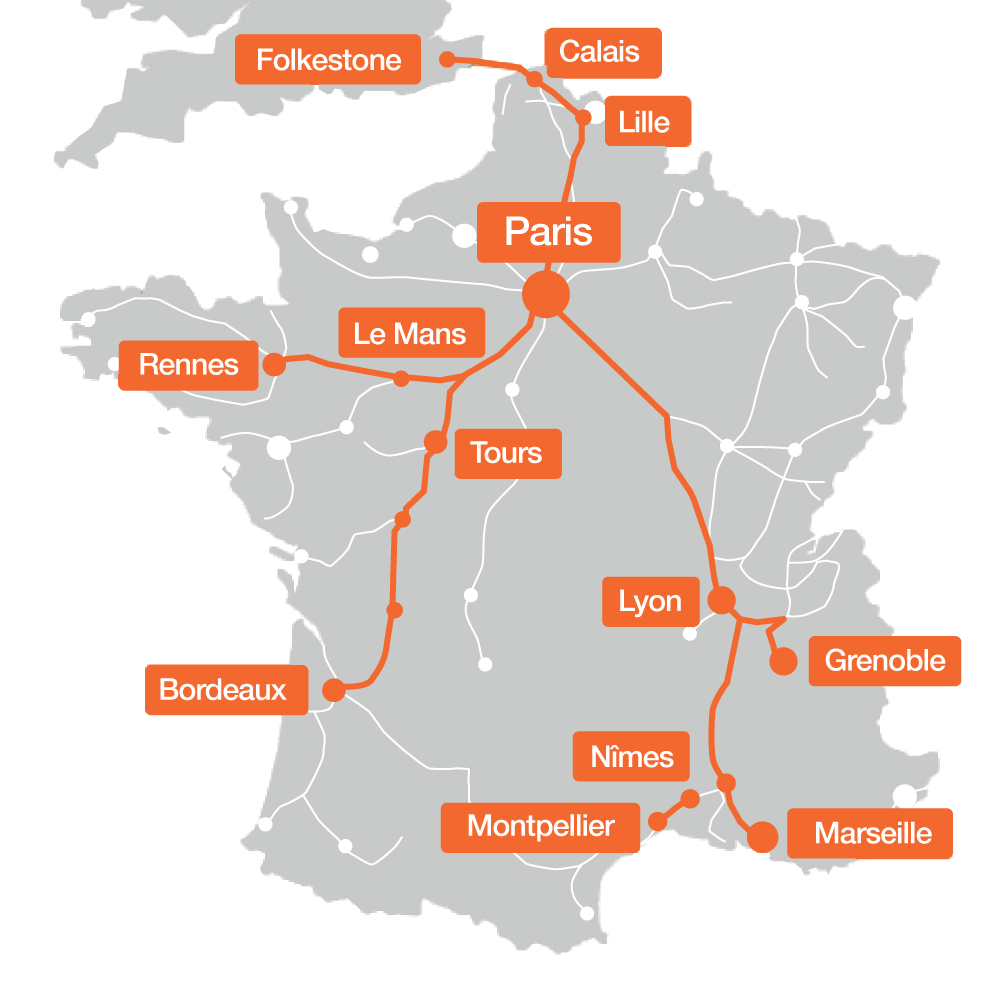
\includegraphics[height=0.3\paperwidth]{images/road\_detection/tgv-4g.png}
                \caption{TGV lines covered in 4G by Orange}
            \end{figure}
        \end{column}
    \end{columns}        
\end{frame}

